\documentclass{article}
\usepackage{tikz}
\usetikzlibrary{arrows.meta}

\begin{document}

\begin{figure}[h]
    \centering
    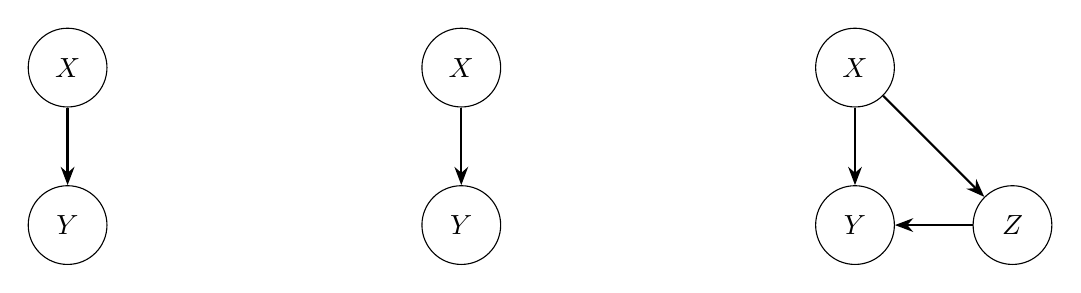
\begin{tikzpicture}[node distance=2cm, auto]
        % Define node styles
        \tikzset{
            vertex/.style = {draw, circle, minimum size=10mm},
            arrow/.style = {-Stealth, thick}
        }
        
        % Nodes
        \node[vertex] (X1) {$X$};
        \node[vertex, below of=X1] (Y1) {$Y$};
        \node[vertex, right of=X1, xshift=3cm] (X2) {$X$};
        \node[vertex, below of=X2] (Y2) {$Y$};
        \node[vertex, right of=X2, xshift=3cm] (X3) {$X$};
        \node[vertex, below of=X3] (Y3) {$Y$};
        \node[vertex, right of=Y3] (Z3) {$Z$};
        
        % Arrows
        \draw[arrow] (X1) -- (Y1);
        \draw[arrow] (X2) -- (Y2);
        \draw[arrow] (X3) -- (Y3);
        \draw[arrow] (X3) -- (Z3);
        \draw[arrow] (Z3) -- (Y3);
        
    \end{tikzpicture}
    
    \caption{Structural causal models (SCMs) represented as directed acyclic graphs (DAGs). Variables are the nodes of the graph and causal effects are represented by arrows. An intervention is an operation that modifies the graph in some way. Intervening on a variable means we erase the arrows pointing into that variable, set the value of that variable arbitrarily, and then propagate the new value along directed pathways pointing out of that variable. On the left, $X$ is a cause of $Y$, so intervening on $X$ will result in a change in $Y$. In the other cases, intervening on $X$ results in no change in $Y$. It is possible that the accuracy of some function $f(X)$ in predicting $Y$ is equal in all cases.}
\end{figure}

\end{document}